\documentclass[11pt,twoside,a4paper]{book}
\usepackage[T1]{fontenc}
\usepackage[utf8]{inputenc}
\usepackage[acronym,toc,xindy]{glossaries}
\usepackage[hidelinks]{hyperref}
\usepackage{geometry}
    \geometry{
     a4paper,
     total={140mm,217mm},
     left=35mm,
     top=40mm,
     }
\usepackage{enumitem}
\setlist{nosep}
\usepackage{graphicx}
\usepackage{setspace}
\usepackage{todonotes}
\usepackage{emptypage}
\usepackage{csquotes}
\usepackage{listings}
\usepackage{longtable, array, booktabs}
\usepackage{csvsimple}

% configure glossary and acronyms
\loadglsentries{glossary.tex}
\loadglsentries{acronyms.tex}
\makeglossaries{}

% overall configurations
\singlespacing{}
\graphicspath{ {images/} }
\newcommand{\porras}[1]{\todo[backgroundcolor=blue!25,inline]{#1}}
\newcommand*{\headentry}[2]{\multicolumn{1}{#1}{\centering\arraybackslash\bfseries #2}}
\renewcommand{\contentsname}{Continguts}
\renewcommand{\chaptername}{Secció}

%languages
\lstdefinestyle{XML}
{
	basicstyle=\ttfamily\small,
	showstringspaces=false,
	commentstyle=\color{blue},
	frame=single,
	language=bash,
    tabsize=4,
}

\begin{document}

    % table of contents
    \tableofcontents{}

    % MAIN MEMORY PART
    \chapter{Introducció al projecte}
    \section{Introducció}
\paragraph{}
Aquest projecte neix de les converses amb Enric Mayol, que introdueix l'API\footnote{\label{foot-api}Interfície de programació d'aplicacions} de FamilySearch i proposa realitzar un projecte relacionat amb les dades emmagatzemades per aquesta organització.

\paragraph{}
\porras{Checking my fucking awesome class}
\gls{API}


\chapter{New section}
    \section{Introducció}
\paragraph{}
Aquest projecte neix de les converses amb Enric Mayol, que introdueix l'API\footnote{\label{foot-api}Interfície de programació d'aplicacions} de FamilySearch i proposa realitzar un projecte relacionat amb les dades emmagatzemades per aquesta organització.

\subsection{subSection}
\paragraph{}
Try some text in here

\subsubsection{Introducció}
\paragraph{}
new glossary entry reference for hana \gls{hana}

\paragraph{}
BLA BLA


    \chapter{La genealogia}

    \paragraph{}
    Resultaria estrany realitzar un projecte que parla o tracta la genealogia en tots els seus apartats i no realitzar una petita introducció que exposi en què consisteix aquesta ciència.

    No representa un objectiu del projecte comprendre l’estat actual de la genealogia en el món contemporani, ni el de crear un dibuix detallat de quines lleis en regulen les seves activitats. No obstant això, sí que es creu que donar una petita visió general dels problemes i preguntes que aquesta ciència pretén abordar pot ajudar a lectors del projecte o futurs estudiants a comprendre millor les  limitacions i oportunitats d'aquest sector.

    \section{Què és la genealogia?}

    \paragraph{}
    La \gls{genealogia} (del grec:  \emph{'genea', 'generació'}; i, \emph{'logos', 'coneixement'}) és també coneguda pel nom d’història familiar. Aquesta ciència consisteix en l’estudi de les famílies, el seguiment dels seus llinatges, tant ascendents com descendents i l’estudi de la història de les persones.

    Els genealogistes, o persones dedicades a la genealogia, tant en l’àmbit privat com personal, utilitzen com a recurs d’investigació arxius històrics rics en dades. Exemples d'aquests recursos poden ser les partides de naixement, documents de defunció, registres d’emigració o altres documents informatius del mateix caire.  L'objectiu d'aquests documents és obtenir informació sobre una persona o família per així poder demostrar relacions de parentesc i llinatge o bé, fets empírics relatius a la vida d'un individu en concret.

    Un altre recurs que es veu cada cop més utilitzat és l'anàlisi genètic, mètode que té una rebuda, demanda i interès més elevat en l’àmbit personal, que no pas en el científic. La finalitat principal d'aquest mètode és la d'esbrinar relacions familiars passades i presents de l'individu a través de l'anàlisi dels seus gens.

    Els motius pels quals una persona pot estar interessada a endinsar-se en el món de la genealogia són diversos. Un exemple podria ser el desig de situar la seva família en un marc més ampli dins de la història o bé, el sentiment de responsabilitat de cara a preservar la història familiar per les futures generacions.

    Els aficionats a la genealogia, que la practiquen com a hobby, generalment investiguen la seva ascendència o la d’una persona propera. Per altra banda, els professionals, acostumen a encarregar-se de realitzar recerques genealògiques per tercers, estudiar i ensenyar mètodes de recerca o mantenir les seves pròpies bases de dades.

    Cal entendre que la genealogia no tracta només de recopilar informació sobre el moment històric en què una persona va néixer, viure o morir, sinó també el de recollir informació sobre l'estil de vida que aquella persona va portar, les seves biografies o quins van ser els esdeveniments i motivacions que van conduir i marcar la seva existència. En altres paraules, podríem dir que una part de les preguntes que la genealogia pretén respondre és la de com van viure o quin caràcter van mostrar els nostres avantpassats al viure durant el transcurs d'esdeveniments històrics, com per exemple, la segona guerra mundial.

    Voldríem tancar aquesta secció indicant que si l'interès per la genealogia, ha anat en augment en els últims temps, és en gran part gràcies a la digitalització de documents, fet que ha permès que genealogistes amateurs disposin d’un ventall d’eines molt superior al que van disposar els seus avantpassats i per tant, que les possibilitats de mantenir un arbre familiar o realitzar recerca genealògica quedin a l'abast de tothom.

    \section{El paper de la genealogia en el transcurs de la història}

    \paragraph{}
    Com s’ha comentat en l'apartat anterior, avui en dia la genealogia és una ciència que busca en gran mesura respondre preguntes de caràcter personal, no obstant això, aquest no va ser sempre el seu objectiu principal.

    Històricament, en les cultures occidentals, les persones estaven interessades a mantenir-se ben informades sobre la seva ascendència de cara a fer latents les seves connexions amb nobles i governants. Generalment, la intenció era protegir la seva situació privilegiada o escapar de la precarietat. En aquesta època, el terme genealogia compartia significat amb el d'\gls{heraldica}, terme usat avui en dia per la ciència que estudia els escuts d’armes. Així doncs, fins a finals del segle XIX, la genealogia deixava la seva marca en la història com a eina utilitzada principalment per aquells amb drets de poder o riquesa adquirits a través de l’herència.

    Aquest exemple, que bé ens podria semblar distant en el temps, no és l’única mostra dels impactes històrics relacionats amb aquesta ciència i com veurem a continuació, existeixen altres exemples molt més propers.

    No cal tornar gaires anys enredera per veure com durant l’època de l’alemanya nazi ser capaç de demostrar l’afiliació a la "raça suprema" era necessari per sobreviure o inclòs poder casar-se de forma legal. Per aquest motiu, no ens ha d’estranyar que avui en dia, Alemanya, segueixi sense fer públics la major part dels registres genealògics del segle XX, doncs els fets històrics han portat a percebre la història familiar com un atac, o amenaça, a la privacitat i seguretat de les persones. Les conseqüències d'aquesta època de la història són conegudes per tothom i un no pot evitar entreveure certes relacions amb el camp de la genealogia.

    Per situar un exemple que ens ocupi si pot ser encara més de ple, podem veure el valor de la memòria històrica i dels sentiments d’unió amb els nostres avantpassats arran de la gran quantitat de publicacions i missatges personals, recordant als seus avantpassats i als temps que els va tocar viure, en relació al vuitantè aniversari de l'esclat de la guerra civil espanyola. De fet, Catalunya és un altre clar exemple contemporani, conjuntament amb Alemanya, de com la memòria històrica pot ser present en la cultura, vida i sentiments de bona part d’una nació. Tant en l’àmbit personal, com col·lectiu.

    Així doncs, podem concloure que la genealogia, no tant com a ciència sinó com eina, va desenvolupar, desenvolupa i probablement, seguirà desenvolupant, un paper important en la història de la humanitat. No hem d’oblidar que els problemes racials segueixen molt presents en l'actualitat de les nostres societats, Estats Units, n'ha estat últimament un clar exemple, i que és la raça sinó una característica més de les nostres característiques de naixement, o en altres paraules, de les nostres dades genealògiques.

    \section{Les lleis reguladores}

    \paragraph{}
    Les seccions anteriors han introduït i descrit les ocupacions principals de la genealogia en els àmbits professional i amateur, així com el paper d'aquesta en la història. També s'ha esmentat que moltes de les dades amb les quals aquesta ciència interactua són de caràcter personal i per tant, sensibles a un ús impropi si no són regulades i protegides sota certes circumstàncies.

    És per aquest motiu que bona part de les dades públiques enregistrades per l’estat, sobretot aquelles que afecten a persones que encara són vives, es troben regulades sota un conjunt de lleis i legislacions. Aquestes lleis varien de nació en nació i per tant, no existeix un estàndard de quina informació és accessible pel domini públic, quina no i sota quines circumstàncies aquesta informació pot ser accedida.

    En el cas de l’estat espanyol són dues les principals lleis que regulen l’accés a les dades genealògiques. La \gls{LOPD} i la legislació consolidada: Llei 20/2011, del 21 de juliol del Registre Civil.

    El registre civil espanyol conté informació detallada d'una persona relacionada amb el seu naixement, relacions d’ascendència i descendència, nom i cognoms, emancipació, declaracions de concurs o suspensió de pagaments, nacionalitat, etcètera, etcètera.  Com podem veure, aquest registre conté tota mena d’informació sensible i al mateix temps, de gran valor de cara a estudis genealògics.

    Els habitants d'Espanya podem demanar accés a l'entrada d'una persona al registre civil mitjançant la presentació d'una sol·licitud digital, escrita o presencial. Per aconseguir aquesta informació caldrà proporcionar tan dades personals pròpies com el motiu pel qual es vol poder accedir a la partida en concret. Motius recurrents són l'estudi genealògic, gestions administratives o simplement la recaptació d'informació.

    Per altra banda, accedir al gruix de la informació no és fàcil i els genealogistes porten xocant amb portes tancades des de fa molts anys. Relacionat amb aquest aspecte, durant l'any 2011 es va aprovar una nova llei del Registre Civil que tenia com a objectiu racionalitzar l'estructura del registre i desjudicialitzar-lo. Aquesta llei havia d'entrar en vigor a partir del 2014, data que va ser posposada fins al juliol del 2015 i recentment ha tornat a ser ajornada fins al 30 de juny del 2017.

    La part que farà referència sobre si el nou registre contemplarà l'accés al públic de cara a la recerca genealògica encara està a l'aire, però sembla que hi ha certa esperança gràcies a la inclusió del següent apartat en l'article 80:

    \begin{displayquote}
        4. Amb caràcter excepcional i amb finalitats d'investigació familiar, històrica o científica, es podrà autoritzar l'accés a la informació registral en els termes que reglamentàriament s'estableixin.
    \end{displayquote}

    Així doncs, sembla que un futur no molt llunyà, aquesta informació podria passar a ser explotable en grans escala de cara a estudis familiars, històrics o científics. Això si, sempre respectant la \gls{LOPD}.

    \section{Els codis ètics en la genealogia}

    \paragraph{}
    El fet que els genealogistes tinguin accés i treballin amb informació pública, però simultàniament, personal, provoca que la professió es vegi envoltada de codis ètics que tractin de protegir la integritat d'aquesta, el sentiment de professionalitat i la moralitat d'aquells que interactuen amb les dades.

    Els codis morals giren al voltant de dos eixos. La protecció de la informació referent a les persones vives i les bones praxis de cara a la manipulació i tractament de les dades.

    El primer eix, tal com hem indicat, fa referència a protegir a aquelles persones que encara són vives. En concret, es tracta d'evitar, en la mesura que sigui possible, publicar informació de caràcter personal que poguí resultar compromesa per un individu en concret.

    El codi moral que hi ha en el rerefons és que a cap persona li agradaria trobar informació personal publicada al núvol, on tothom la pot accedir, pel simple fet que es tracta d'informació `pública'. Per tant, cal respectar la privacitat de les persones i no publicar fets o dades compromeses independentment de l'opinió personal del genealogista.

    Com ja s'ha mencionat amb anterioritat, la genealogia tracta en gran mesura d'estudiar els nostres avantpassats i la història de tots aquells que van existir abans que nosaltres, per tant, el xafardeig i la tafaneria no tenen cabuda dins dels codis ètics i morals de la professió.

    La segona branca ètica es correspon a un seguit de bones praxis de cara a la utilització d'informació genealògica. Tot i que no es tracta d'un manual oficial, la següent llista de `regles' serveix per descriure i fer-nos una idea amb un alt grau de fiabilitat, del que significa el concepte de bones praxis en aquesta ciència:

    \begin{itemize}
        \item El genealogista mantindrà les fonts de referència i les citarà quan utilitzi dades fetes públiques per un altre individual o col·lectiu.
        \item El genealogista no compartirà ni utilitzarà informació no contrastada o amb altes probabilitats de ser errònia.
        \item El genealogista transmetrà seguretat i confiança a aquells que facin ús dels seus serveis.
        \item El genealogista donarà suport a aquelles iniciatives que preservin els fitxers públics i l'accés a aquests.
        \item Es tractarà amb cordialitat i respecte al personal de les facilitats d'investigació.
        \item El genealogista ajudarà en la mesura que sigui possible als altres genealogistes i organitzacions dedicades a la genealogia.
        \item El genealogista compartirà els resultats dels seus estudis i investigacions.
        \item No està permesa la invenció ni exageració de la informació.
        \item El genealogista complirà amb les lleis en rigor dels conjunts de dades que utilitzarà en els seus estudis.
    \end{itemize}

    \section{El procés de recerca genealògica}

    \paragraph{}
    A tota persona que li interessi realitzar recerca genealògica sobre la seva pròpia família o la d'una persona propera, se li suggereix el següent procés com a mètode de treball.

    El procés de recerca es desenvolupa en cicles i cada cicle consta de cinc fases. A continuació es detallen una a una:

    \begin{enumerate}
        \item \textbf{Identificar el que es coneix:} Identificar i revisar tota la informació inicial que es coneix. Pel final de la fase s’haurien de tenir recopilats, ordenats i documentats tots els esdevenimentals relacionats amb la família o persona a estudiar disponibles.
        \item \textbf{Decidir que es vol aprendre:} L’objectiu d’aquesta fase és identificar sobre quin individu es vol obtenir informació, que es vol aprendre d’aquesta persona i si és possible el temps i llocs aproximats en els quals aquesta persona va viure.
        \item \textbf{Seleccionar els arxius a consultar:} Aquesta fase resulta la més complexa de tot el procés. L’objectiu, ordenar de més a menys útils les diferents fonts de dades a consultar i quins arxius resulten més interessants.
        \item \textbf{Obtenir i consultar els arxius:} Durant aquesta fase es consultaran les fonts de dades seleccionades a l’apartat anterior. Al final d’aquesta, hauríem de tenir anotat tot allò que s’ha descobert i còpies dels documents que suporten els descobriments, ja sigui en format de fotocòpies, notes o qualsevol altra mena de suport físic o digital.
        \item \textbf{Utilitzar la informació:} Finalment, en aquesta fase, tocarà avaluar la informació descoberta, transportar la nova informació als formularis adients, organitzar la informació i compartir els resultats. Un cop finalitzades totes aquestes tasques s'estarà preparat per tornar a iniciar la roda del procés i seguir així amb la recerca genealògica.
    \end{enumerate}

    \paragraph{}
    La figura~\ref{fig:researchProcess} mostra les cinc fases d'aquest procés cíclic.

    \begin{figure}[h]
            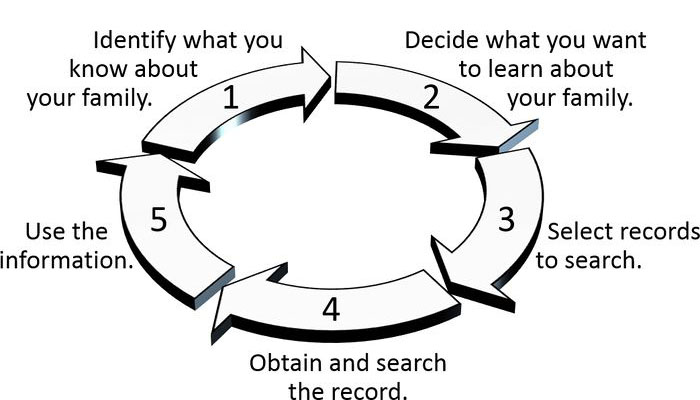
\includegraphics[scale=0.6]{02/researchProcess}
            \centering
            \caption{Procés de recerca genealògica.\label{fig:researchProcess}}
    \end{figure}

    \section{Conclusió}

    \paragraph{}
    Donem d'aquesta forma per conclosa la breu introducció a la genealogia. Com s'ha pogut observar, es tracta d'una ciència d'especial vocació personal, amb regulacions ambigües i rodejada de codis ètics i morals.

    Tot i les dificultats que tant genealogistes amateurs com professionals poden haver de fer front, aquesta ciència és capaç de desemmascarar i ajudar a comprendre les vivències dels nostres avantpassats i crear així un enllaç entre passat, present i futur. 


    \chapter{L'organització FamilySearch}
    \paragraph{}
    En aquest apartat de la memòria s'introduirà l’organització de FamilySearch. En concret, s’explicaran els objectius i motivacions sota les que va néixer l’organització, la seva història i el conjunt de funcionalitats i serveis que ofereixen a través del seu portal web i centres d’investigació.

    \section{Què és FamilySearch?}

    \paragraph{}
    Si haguéssim de resumir l’organització en una sola paraula, aquesta seria família. Com s’indicava en la introducció, FamilySearch és una organització sense ànim de lucre destinada  connectar famílies a través de diferents generacions. Des de l’organització es creu que les famílies són un condicionador de la felicitat i un dels factors que donen sentit a la vida.

    La seva visió com a empresa, amb les seves pròpies paraules, és:

    \begin{displayquote}
        Aprendre dels nostres avantpassats, a través dels llaços familiars, ens ajudà a comprendre millor qui som, enllaçar el present amb el passat i construir els ponts cap al futur.
    \end{displayquote}

    Aquesta visió és perseguida mitjançant un equip de professionals i voluntaris que treballen de cara a preservar i compartir el que s'ha convertit en la col·lecció més gran del món d'arxius genealògics. Aquest fet no és fruit de la casualitat, sinó dels més de cent anys que aquesta organització porta recol·lectant, preservant i compartint arxius genealògics des de tots els indrets del globus terraqüi.

    FamilySearch organitza i tracta els recursos disponibles tenint present que la finalitat de les dades és poder ser consumides per tercers. Per això, FamilySearch aposta per un model de dades eficaç, on aquelles persones interessades a explorar el seu passat, puguin descobrir amb certa facilitat quin són els seus orígens.

    Algunes de les característiques o dades que ajuden a comprendre l'envergadura i èxit d’aquesta organització se citen a continuació:

    \begin{itemize}
        \item Servei gratuït.
        \item Més de 4 bilions de persones diferents emmagatzemades en el sistema. Per tenir una idea de la magnitud d'aques nombre, actualment s’estima que en el món viuen 7,4 bilions de persones.
        \item 4.765 centres d’investigació distribuïts arreu del món.
        \item Servei d'ajuda 24/7.
    \end{itemize}

    \section{La història de FamilySearch}

    \paragraph{}
    FamilySearch, en els seus orígens coneguda com la Societat Genealògica de Utah, va néixer de les mans de l'església de Jesucrist dels Sants dels Darrers Dies l'any 1894. Aquesta església també és coneguda avui en dia pel nom de l'església mormona.

    L’organització porta acumulats a les seves espatlles més de cent anys de recerca i preservació d’arxius històrics i genealògics. Durant aquest recorregut, FamilySearch s’ha associat amb més de 10.000 arxius i 200.000 voluntaris de tota mena d’indrets.

    Mitjançant l’esforç col·lectiu d’aquestes organitzacions s’ha aconseguit preservar tant índexs com imatges d’arxiu de gran qualitat i posar tots aquests recursos a la disposició de milions de persones de forma gratuïta.

    Durant aquest trajecte de més de 100 anys iniciat l'any 1894, l'organització ha tingut l'oportunitat de celebrar grans èxits. Entre ells, destaquen els següents:

    \begin{itemize}
        \item \textbf{1938, Microfilm:} La societat genealògica de Utah és pionera en començar a utilitzar microfilm per filmar i emmagatzemar informació relativa a arxius genealògics arreu del món.
        \item \textbf{1942, Family group record archive:} Es crea, de forma manual, una indexació de les genealogies compartides fins aquell moment.
        \item \textbf{1963, Baül d’arxius a les Granite Mountains:} Es completa la creació d’un baül d’arxius amb tecnologia punta situat a les muntanyes pròximes a Salt Lake City, Utah, indret on resideix, avui en dia, la seu de l’organització. Es tracta d’una instal·lació climatitzada que ha estat utilitzada des de la seva creació per preservar còpies de microfilm i arxius digitals de més de cent països diferents.
        \item \textbf{1970, Primers centres d'història familiar:} S'introdueixen els primers centres d'història familiar. Aquests centres formen part d'una ramificació de llibreries que ofereixen accés gratuït a la informació continguda per més de 2,4 milions d'arxius en microfilm. Com hem esmentat en l'apartat anterior, avui en dia existeixen 4.765 d'aquests centres.
        \item \textbf{1985, L’estàndard GEDCOM:} En aquest any FamilySearch introdueix l'estàndard de \gls{GEDCOM}. L'estàndard GEDCOM consisteix en un conjunt d'especificacions i regles sobra com s'ha d'estructurar la informació genealògica de cara a compartir-la amb facilitat a través del núvol.
        \item \textbf{1995, Arbres genealògics digitalitzats:} Es dóna l’oportunitat als genealogistes de digitalitzar els arbres genealògics a la seva disposició i habilitar-ne l’accés a altres usuaris.
        \item \textbf{1998, Digitalització d’imatges:} FamilySearch comença a utilitzar tecnologies d'imatge digital per tal de capturar noves fonts de dades i transformar els milions de continguts, emmagatzemats fins ara en microfilm, en imatges digitals. La tecnologia també permet crear índexs de fàcil utilització que relacionen persones amb els continguts digitals.
        \item \textbf{1999, Nova pàgina web:} La pàgina web FamilySearch.org arriba al núvol. En la seva fase inicial, aquesta oferia la possibilitat de cercar informació en els registres històrics de forma relativament simple.
        \item \textbf{2012, Noves tecnologies digitals:} S’incorpora a les tecnologies utilitzades per FamilySearch la tecnologia dCamX, utilitzada per la digitalització de documents i la creació de  sales de lectura digital, responsables de facilitar les tasques de comunicació i alliberació de coneixement entre els diferents centres.
    \end{itemize}

    Un dels altres grans èxits de  l’organització, del que malauradament no es coneix la data exacte de creació, va ser \textbf{l’obertura de la FamilySearch \gls{API}.}

    Aquesta va suposar que aplicacions externes poguessin connectar-se a les bases de dades de FamilySearch i utilitzar-ne la informació d'una forma regulada i eficient. Resulta prou evident que sense l'existència d'aquesta \gls{API}, aquest projecte mai hagués pogut tenir lloc.

    \section{L'església mormona i la família}

    \paragraph{}
    Ja que el principal benefactor de FamilySearch és l'església mormona, creiem que és interessant estudiar de forma breu els orígens d'aquesta.

    L’església de Jesucrist dels Sants dels Darrers Dies és una església que considera que la religió hauria de tornar als seus inicis apostòlics. Va ser fundada pel nord-americà Joseph Smith el 6 d’abril del 1830, a l'oest de Nova York.

    Considerada actualment com la quarta comunitat cristiana més gran als Estats Units, troba situada la seva seu en l'actualitat a Salt Lake City, Utah. No obstant això, durant els inicis de l’església, Smith tenia la intenció de crear la Nova Jerusalem a prop de Nova York, en una ciutat que anomenaria \emph{Zion}.

    L’església, amb origen als voltants de Nova York, es va desplaçar cap a Kirtland, Ohio, des d'on va començar a expandir-se per Jackson County, Missouri, terra en què Smith volia situar la seu del col·lectiu en un futur pròxim.

    Joseph va veure contrariats els seus plans, quan l'any 1833, els colons van expulsar brutalment al col·lectiu de Missouri. Com que no disposaven dels recursos militars necessaris per recuperar el territori per la força, es van veure obligats a anar desplaçant-se al llarg de diferents localitzacions, sempre per culpa de conflictes amb els natius de les terres, fins a establir-se a Nauvoo, Illinois.

    Després de la mort de Smith, per tal d'evitar els conflictes armats amb els residents d'Illinois, el col·lectiu es va desplaçar cap a Nebraska i més endavant, durant l'any 1847, a les terres que serien conegudes com a Utah.

    Durant aquesta època, l'església es va veure sotmesa a grans pressions i crítiques a causa de la seva tolerància per la poligàmia. Les tensions entre el col·lectiu i el govern d'Estats Units anirien en augment, fins que l'any 1890, el congrés va disgregar l'església i es va apoderar de molts dels seus béns.

    Arribats aquest punt, l'església fundada per Smith, va decidir deixar de donar suport als matrimonis plurals, però sense desfer les famílies que ja es trobaven unides sota aquestes condicions.

    Durant el segle XX, l'església va créixer substancialment i es va veure sotmesa a un procés d'internacionalització, en gran mesura, gràcies a la feina dels missioners enviats a diferents indrets del món.

    Durant aquest període el col·lectiu es va convertir en un ferm defensor de les famílies nuclears, és a dir, de les famílies que consisteixen en dos progenitors i la seva descendència. L'església també va oposar-se en aquesta època a l'esmena pels drets igualitaris entre homes i dones, els casaments entre persones del mateix sexe i l'eutanàsia.

    Hem volgut redactar aquests paràgrafs previs sobre els orígens de l'església mormònica per tal de poder presentar, amb cert rigor històric, com l'església va veure canviat i evolucionat el concepte de família al llarg del temps.

    També queda latent, d'aquesta forma, com la història del col·lectiu es va veure marcada pel rebuig i el desterrament de moltes terres, fins al punt que van haver de recórrer a l'ús de missioners, repartits arreu del món, per tal de sobreviure com a religió.

    Així doncs, creiem que per aquest projecte no esdevé necessari entrar en més detall pel que fa a les doctrines i pràctiques de l'església, ni  enumerar quines són les principals diferencies entre l'església mormona i les altres corrents del cristianisme. Per altra banda, sí que volem realitzar una reflexió final sobre la posició actual de l'església mormona respecte a la família.

    Pels mormons, les famílies representen els lligams que uneixen a les persones en relacions personals i les connecten tant amb les passades com amb les futures generacions. Creuen que cap èxit en la vida, pot compensar el fracàs en l'àmbit familiar.

    Segons el seu punt de vista, construir nuclis familiars units i forts és el remei a molts dels fracassos que tenim les persones com a societat i creuen que la família inspira a l'individu a pensar més enllà de l'interès propi o la gratificació immediata i l'anima a entregar-se per altres persones, comunitats i a déu.

    Forma part també de la cultura mormona la pràctica o deure d'acumular i preservar, tant les històries dels seus avantpassats com les pròpies, en benefici d'aquells que encara estan per arribar, enllaçant, d'aquesta forma, generacions desconnectades d'una altra forma.

    Entenen la naturalesa real de la família, com un algú que transcendeix l'aquí i l'ara i que permet a les persones extreure forces d'aquells que van viure abans que nosaltres.

    Concloïen, si ajuntem les dues variables que van marcar l'esdevenir de l'església mormona fins als temps contemporanis, és a dir, la seva semi forçada internacionalització i la importància del nucli familiar en la seva cultura, no hauríem de mostrar-nos sorpresos pel fet que el col·lectiu s'hagi convertit en un dels referents mundials en el camp de la genealogia.

    \section{Serveis per organitzacions amb arxius genealògics}

    \paragraph{}
    Com ja s’ha comentat en seccions anteriors, FamilySearch no és només una organització dedicada a posar a disposició del públic registres genealògics, sinó que també pretenen ajudar a altres organitzacions a digitalitzar i publicar els seus documents al núvol de forma econòmica, ja sigui mitjançant la plataforma FamilySearch o la construcció de noves eines pròpies al núvol.

    Sigui com sigui, FamilySearch ofereix cinc serveis a altres organitzacions genealògiques:


    \subsection{Captura d'imatges}

    \paragraph{}
    Obtenir imatges de qualitat és normalment el procés més costos per aquelles organitzacions que volen digitalitzar els seus registres, tant en el sentit econòmic, com en base als recursos humans necessaris.

    El microfilm, que fins fa poc era l’estàndard en la indústria, comença a cedir pas al món digital i tant si l’objectiu de les organitzacions és digitalitzar el seu contingut mitjançant medis propis o utilitzant la tecnologia disponible en els centres de recerca de FamilySearch, aquests ofereixen la seva ajuda a les organitzacions que la sol·licitin.

    La tecnologia dCamX, utilitzada per FamilySearch, es caracteritza per la creació d'imatges d’alta qualitat, de forma eficaç, al mateix temps que es capturen meta dades de la imatge. Aquest aspecte, conjuntament amb un procés de publicació posterior fàcil i ràpid, fan que aquesta tecnologia estigui cridada a ser el nou estàndard a la indústria.


    \subsection{Conversió de formats digital}

    \paragraph{}
    Aquest servei està pensat per aquelles empreses o organitzacions que ja disposen d’una elevada quantitat de material en format de microfilm.

    La tecnologia digital ha canviat dràsticament com els registres són capturats, emmagatzemats i fets accessibles. Aquesta tecnologia segueix progressant i per tant resulta indispensable començar a adaptar-se al més aviat possible.

    FamilySearch posa a disposició de les organitzacions genealògiques la possibilitat d’utilitzar els mateixos processos i software que utilitzen ells per digitalitzar la seva col·lecció de més de 2,4 milions de microfilms. FamilySearch, també ofereix la possibilitat d’emmagatzemar els fitxers digitals d’aquestes organitzacions en els seus servidors, un cop convertits, si així ho prefereixen.


    \subsection{Indexació en línea}

    \paragraph{}
    Un cop un registre ha estat digitalitzat en forma d’imatge, la informació principal necessita ser extreta i transcrita per tal de poder produir índexs sobre els quals clients o usuaris puguin cercar.

    L’aplicació d’indexació en línea, creada per FamilySearch, permet, mitjançant la cadena de voluntaris, crear índexs de forma ràpida i precisa. Els arxius de les organitzacions, que així ho sol·licitin, podran disposar d’accés a aquesta cadena de voluntaris per digitalitzar els seus índexs o accés a les eines d’indexació auxiliars  que permeten la creació de projectes propis.


    \subsection{Accés en línea}

    \paragraph{}
    Si un document o registre no esdevé fàcilment accessible, resulta de poc valor pels usuaris. FamilySearch ofereix dos serveis diferents depenent de si les organitzacions desitgen fer públic l'accés a les seves dades a través de FamilySearch.org o no.

    En cas de voler per públics els registres, FamilySearch s’ofereix a penjar i mantenir els registres de forma econòmica. En cas de voler mantenir els registres en un àmbit privat, l’organització posa a disposició dels interessats les eines i experiència necessàries per crear un espai propi al núvol.


    \subsection{Preservació dels registres i fitxers físics}

    \paragraph{}
    FamilySearch ofereix l’opció a les organitzacions de custodiar còpies de seguretat dels seus fitxers, en el baül de tecnologia punta situat a las Granite Mountains. En l'actualitat, còpies d’arxius de microfilm i digitals, provinents de més de cent països diferents, es troben guardades en aquest baül per precaució.

    El fet de disposar de còpies de seguretat pels fitxers genealògics, suposa la salvació de registres en cas de terratrèmols, incendis, inundacions, tornados, guerres i actes humans no controlables en les seus oficials dels arxius.

    Les mesures de seguretat que FamilySearch utilitza pels seus registres i que a la vegada, queden a disposició d’altres organitzacions, són:

    \begin{itemize}
        \item Processos complets i automatitzats de comprovació, validació i actualització dels registres per garantir la màxima protecció possible.
        \item Migració gradual i eficient de registres cap a noves tecnologies quan els formats previs quedin obsolets, garantint així la seva accessibilitat a llarg termini.
        \item Processos de conversió i preservació de dades que compleixen amb les regulacions sobre els \gls{OAIS}.
        \item Col·leccions d’informació emmagatzemada al núvol i distribuïdes en diferents clústers arreu del món per garantir una alta capacitat d’emmagatzematge, escalabilitat i protecció contra els desastres.
        \item Utilització de les últimes tecnologies en el tractament de dades d'alta densitat.
        \item Procés ràpid i eficient de cara a processar l'arribada de nous registres al sistema. El sistema actual és capaç de processar més de vint terabytes al dia, mesura que incrementa, al mateix temps que la tecnologia avança.
        \item Servidors configurats en clústers virtuals per garantir una escalabilitat infinita.
        \item Facilitat amb control climàtic, prevenció de focs, fonts d’energia auxiliars per casos d’emergència i replicació d’arxius digitals.
    \end{itemize}


    \subsection{Conclusions sobre els serveis professionals}

    \paragraph{}
    En els apartats anteriors s'ha pogut observar com FamilySearch està clarament interessada a posar les seves tecnologies a disposició d'altres organitzacions genealògiques.

    Aquesta estratègia de col·laboració els permet incorporar a les seves bases de dades registres d'informació, d'altre forma inaccessibles i garantir la persistència de les dades davant d'esdeveniments no controlables, d'informació gestionada per altres organitzacions.


    \chapter{Introducció a l'API de FamilySearch}

    \section{El portal de desenvolupadors}

    \paragraph{}
    Tota la informació disponible per tal de poder començar a familiaritzar-se amb l’\gls{API} de FamilySearch, pot ser trobada en el portal de desenvolupadors.

    Aquest apartat de la web està format per diferents seccions, malauradament, l’estructura no acaba de resultar del tot clara per una persona que vulgui iniciar-se per primer cop en l'ús d'aquesta \gls{API}.

    Si ens enfoquem més en la documentació disponible, que no pas en l'estructura proposada per l’organització, podem veure que la informació es podria distribuir, en certa forma, en els següents grups:

    \begin{itemize}
        \item \textbf{Requisits tècnics:} Conjunt d’informació necessària per comprendre l’estructura de l'\gls{API}, els formats de dades que maneja i els passos necessaris per començar a interactuar amb aquesta.
        \item \textbf{Recursos disponibles i rutes d’accés:} Informació detallada sobre cada recurs accessible a través de l'\gls{API}. En concret, disposa dels detalls de com accedir al recurs, les operacions que es poden realitzar sobre ell, la informació que conté i quines són les connexions amb altres recursos.
        \item \textbf{Evolució i canvis produïts a l'\gls{API}:} Informació semi ordenada de com l'\gls{API} s’ha vist evolucionada al llarg del temps i un recull dels canvis produïts sobre els recursos, procés de certificació, material de documentació i eines de desenvolupament.
        \item \textbf{Serveis extres oferts per l'\gls{API}:} Aquest recull d’articles conceptualitza característiques de l'\gls{API} com poden ser els recursos d'\emph{emmagatzematge}, \emph{localització} o \emph{throttling}.
        \item \textbf{Eines de desenvolupament:} Recull d’entorns de desenvolupament i eines extres que poden facilitar la feina del desenvolupador.
        \item \textbf{Certificació:} Recull la informació necessària per gestionar els diferents processos de certificació i informació sobre les regulacions a les quals s'ha de fer front en cas de voler certificar l'aplicació.
    \end{itemize}

    \section{L'arquitectura de l'\gls{API}}


    \subsection{Què és una \gls{API}?}

    \paragraph{}
    Abans d'entrar en detall en com funciona una \gls{API}, estaria bé definir, amb una mica més de precisió, en què consisteix exactament.

    Una \gls{API}, de l'anglès `Application Programming Interface' o Interfície de programació d'aplicacions en català, representa el conjunt de subrutines, funcions i procediments que ofereix una biblioteca per tal de ser utilitzada en el software de tercers com una capa d'abstracció. Aquest conjunt de subrutines, funcions i procediments, acostumen a oferir accés a certs serveis o conjunts de dades d'un particular, a tercers, de forma controlada.


    \subsection{L'arquitectura REST}

    \paragraph{}
    L’arquitectura sobre la qual està creada l’\gls{API} de FamilySearch és una arquitectura REST. Les sigles provenen de l’anglès i representen el concepte: \gls{REST}.

    Les arquitectures \gls{REST} es caracteritzen per estar orientades els recursos més que a les accions que es poden realitzar sobre ells i com a peculiaritat, es caracteritzen per sis regles o restriccions.

    Aquestes són: interfície uniforme, sense estat, client-servidor, emmagatzemables, sistema per capes, i codi sota petició. Aquests sis conceptes són doncs els que defineixen les bases de es arquitectures \gls{REST}.

    És diu que una arquitectura \gls{REST} és orientada als recursos perquè estan construïdes al voltant d’objectes i les relacions entre aquests, en comptes d’accions. Per exemple, a l’\gls{API} de FamilySearch, es parla de persones i esdeveniments, en comptes de llegir persones o crear esdeveniments i en canvi, aquestes operacions, passen a formar part dels objectes \emph{Persona} i \emph{Esdeveniment.}

    L'intercanvi de dades es produeix mitjançant l'ús de diferents representacions. Aquestes, expliquen com els recursos són tractats per l’\gls{API} i de quina forma han de ser realitzades les comunicacions entre el servidor i el client. Els formats més freqüents són JSON i XML. FamilySearch ofereix suport per ambdós formats.

    Per posar un exemple reduït que il·lustri el que estem explicant, podem descriure de la següent forma, el que podria ser una operació contra l'\gls{API} de FamilySearch, especificant quin element seria considerat el Recurs, quin el Servei i quin la Representació:

    \begin{itemize}
        \item \textbf{Recurs:} Persona (informació relacionada amb una persona en concret)
        \item \textbf{Servei:} Obtenir informació de la persona (GET)
        \item \textbf{Representació:} Nom, cognoms, esdeveniments relacionats amb la vida de la persona, etcètera, en format \gls{XML} o \gls{JSON}.
    \end{itemize}

    \paragraph{}
    Com també s'ha comentat, l’arquitectura \gls{REST} es caracteritza per la implementació de sis restriccions imposades sobre el sistema. A continuació s'exposa amb més detall, cada una d'elles.


    \subsubsection{Interfície uniforme (uniform interface)}

    \paragraph{}
    Aquesta restricció s'encarrega de definir la interfície de comunicació entre el client i el servidor.

    En una arquitectura REST, s'utilitzen els protocols de comunicació \gls{HTTP} i \gls{HTTPS} de forma conjunta amb els \gls{URI}, per aconseguir accés als diferents recursos i operacions proporcionades per l'\gls{API}.

    Els verbs permesos pels protocols de comunicació web són els coneguts: get, put, post, delete, options and head.

    Per exemple, per fer la petició de lectura sobre el recurs d’una Persona a l’\gls{API} de FamilySearch, executaríem la següent crida \gls{HTTP} o \gls{HTTPS} mitjançant el verb i URI especificats a continuació:\\ \verb|GET /platform/genealogies/persons/2:2:PPPJ-MYZ7|.


    \subsubsection{Sense estat (stateless)}

    \paragraph{}
    Aquesta restricció implica que el servidor no emmagatzema la informació del client. Això implica que cada petició d'aquest cap a l’\gls{API}, ha de contenir tota la informació necessària perquè el servidor l'identifiqui i es defineixin les regles de comunicació adequades per processar la petició.

    Hi ha exemples d'operacions a l'\gls{API} de FamilySearch, com per exemple el procés d'identificació Oauth V2, que no són realment RESTful, doncs aquestes sí que guarden informació del client durant les diferents parts de la comunicació.


    \subsubsection{Client-servidor (client-server)}

    \paragraph{}
    Per comprendre aquesta restricció, cal comprendre primer en què consisteix un sistema desconnectat.

    En el cas de les arquitectures REST, un sistema desconnectat implica que el client mai tindrà accés directe a les bases de dades que emmagatzemen la informació, i que per tant, sempre haurà d'accedir a les dades mitjançant l’intermediari. En aquest cas, l'\gls{API}.

    Els protocols de comunicació descrits prèviament (\gls{HTTP} i \gls{HTTPS}), i la interfície de comunicació, són els encarregats de gestionar les comunicacions entre client i servidor.


    \subsubsection{Emmagatzematge en el client (cacheable)}

    \paragraph{}
    Aquesta restricció fa referència a si les respostes retornades, des del servidor, al client, poden ser emmagatzemades per aquest i durant quant de temps les pot guardar. Existeixen tres nivells de configuració diferents:

    \begin{itemize}
        \item \textbf{Implícit:} Si és el client el que decideix quant de temps guardarà les dades o informació retornada, es tracte d'emmagatzematge implícit.
        \item \textbf{Explícit:} Si és el servidor el que mana i posa les regles, parlem d'emmagatzematge explícit.
        \item \textbf{Negociat:} Quan el client i el servidor negocien i arriben a un acord, es tractea d'emmagatzematge negociat.
    \end{itemize}


    \subsubsection{Sistema per capes (layered system)}

    \paragraph{}
    Aquest principi, o restricció, es basa en el fet que el client no pot assumir que tindrà connexió directa amb el servidor. És a dir, poden existir diferents intermediaris en forma de hardware i software entre client i servidor.

    Això, facilita l’escalabilitat i persistència del sistema gràcies al fet que el client no s’ha de preocupar de comunicar-se amb elements o tecnologies específiques. D'aquesta forma, el servidor es pot veure subjectes a canvis de forma transparent pels clients.


    \subsubsection{Codi sota petició (code on demand)}

    \paragraph{}
    Restricció que regula com, de forma excepcional, el servidor pot proporcionar accés al client sobre certes parts de la lògica del funcionament. Alguns exemples poden ser els \emph{Java Applets} o blocs de codi \emph{JavasScript}.

    \section{Formats de dades utilitzats pel Sistema}

    \paragraph{}
    FamilySearch utilitza tres formats de dades diferents per representar la informació emmagatzemada en les seves bases de dades i dos formats extres per codificar aquesta informació i enviar-la a través del núvol.

    Els conjunts de dades utilitzats per representar els recursos són els que segueixen:

    \begin{itemize}
        \item Les dades genealògiques es representen mitjançant el format GEDCOM X.
        \item Els recursos o objectes específics del model de FamilySearch, es representen mitjançant una extensió del model de dades GEDCOM X.
        \item El format de dades Atom, o atòmic, s’utilitza per proporcionar un format simple per les meta-dades.
    \end{itemize}


    \subsection{El format de dades GEDCOM i GEDCOM X}

        \paragraph{}
        El terme \gls{GEDCOM}, és un acrònim de l'anglès Genealogical Data Communications.

        El format GEDCOM consisteix en un conjunt de regles d'aplicació per tal de representar informació genealògica. Aquest format de dades, creat per FamilySearch l'any 1984, s'ha convertit en l'estàndard de la indústria.

         Per simplificar-ho, podríem entedre un fitxer en format GEDCOM, com un fitxer de text que emmagatzema informació genealògica d’una persona i les metadades necessàries per poder enllaçar als diferents fitxers de la mateixa persona.

         Tot i que l’última versió, datada del 1996, segueix sent molt utilitzada, FamilySearch va proposar durant l'any 2012, canviar aquest estàndard per la seva nova versió anomenada GEDCOM X.

         El format de dades per la \gls{GEDCOM X}, representava un nou projecte de codi obert i es diferenciava del seu antecessor en la implementació d'un sistema que facilitava la inclusió d'arbres genealògics i fonts de dades als recursos ja existents.

         Al mateix temps, el nou estàndard també donava suport a l'intercanvi i enllaçament de dades a través del núvol i es creava així la primera versió de l'API de FamilySearch.

         A continuació, a la taula [ref] s'ofereix un petit exemple de com un recurs és codificat part del recurs persona sota el format de dades GEDCOM X.

        \begin{center}
                 \csvreader[
                    separator=comma,
                    before table=\sffamily\small,
                    longtable={p{1.5cm-2\tabcolsep}p{4.5cm-2\tabcolsep}p{4.5cm-2\tabcolsep}p{3.5cm-2\tabcolsep}},
                    table head={\toprule%
                        \headentry{m{1.5cm-2\tabcolsep}}{Nom}
                        & \headentry{m{4.5cm-2\tabcolsep}}{Desc.}
                        & \headentry{m{4cm-2\tabcolsep}}{Format}
                        & \headentry{m{4cm-2\tabcolsep}}{Rest.}\\\midrule},
                    late after line=\\\midrule,
                    late after last line=\\\bottomrule,
                 ]
                 {./tables/04/gedcomFinal.csv}
                 {nom=\nom,desc=\desc,format=\format,rest=\rest}
                 {\nom&\desc&\format&\rest}
         \end{center}

         \paragraph{}
         Així doncs, podem veure com la instància del recurs Persona conté un camp booleà, que indica si aquesta pot ser utilitzada de forma pública o només en l'àmbit privat i tres camps que es troben codificats sota els estàndards del format GEDCOM X.

         Per exemple, el format de dades \verb|http://gedcomx.org/v1/Gender|, representaria un recurs amb l’estructura que s’exposa a la taula [ref2] i els valors possibles per l’enumeració de gènere, s’indiquen en la taula [ref3]

         [TABLE 2]

         [TABLE 3]

         \paragraph{}
         Com que l’objectiu del projecte no és estudiar la codificació GEDCOM o GEDCOM X, sinó comprendre quina informació es troba realment disponible a través de l'API de FamilySearch, no entrarem més en detall en aquests formats.

         L’objectiu d’aquest apartat era explicar quin és l'estàndard de representació de dades genealògiques utilitzat per l'API. Per qualsevol informació extra que es vulgui consultar, s’adjunta a la bibliografia del projecte, l’enllaç a la documentació del model conceptual.


     \subsection{Format de dades FamilySearch}

        \paragraph{}
        El format de dades FamilySearch, defineix el format d'aquells objectes específics relacionats amb la plataforma de dades pròpia de l'organització. Això implica que aquestes estructures no formen part de cap estàndard i manquen de sentit fora del context pel qual han estat definides.

        L'estructura dels objectes específics de FamilySearch ha estat creada com una extensió de l'especificació GEDCOM X. Per tant, segueixen una estructura molt similar.


    \subsection{Format de dades Atom (o Atòmic)}

        \paragraph{}
        Els formats de dades Atom, o atòmic, és utilitzat per proporcionar un format pel contingut web i les metadades.

        Aquest format és utilitzat, entre altres llocs, en les col·leccions ordenades de resultats, com podrien, per exemple, les respostes a la funció de cerca de persones o l'obtenció del historial de canvis d’una persona.


    \subsection{Codificacions dels formats de dades}

        \paragraph{}
        Els formats de dades que s’han exposat en els apartats anteriors no són més que unes convencions que marquen l'estructura a seguir per representar els diferents objectes o recursos utilitzats per l'API de FamilySearch.

        Tanmateix, aquestes estructures han de ser codificades per tal de poder ser transmeses a través del núvol i en concret, FamilySearch, proporciona suport a les dues codificacions més comunes i utilitzades per aquesta finalitat. Els llenguatges XML i JSON.


        \subsubsection{El llenguatge XML}

        \paragraph{}
        El \gls{XML}, és un llenguatge de marcatge que defineix un conjunt de regles a seguir per tal de codificar, documents i informació, en un format llegible i processable, tant per éssers humans, com màquines.

        El llenguatge va ser definit pel Consorci World Wide Web i tracta d’emfatitzar la simplicitat, generalitat i usabilitat del model, per l'ús a través d'Internet.

        Una versió reduïda de la representació en XML del recurs ‘Nota’, amb camps: subjecte, text i atribució, quedaria representat de la forma següent:

        \begin{lstlisting}[style=rawOwn,caption={Representació bàsica en XML d'una Nota}]
<Note xmlns='...'>
    <subject>...</subject>
    <text>...</text>
    <attribution id='...'>
        <contributor resourceId='...' resource='...'/>
        <modified>...</modified>
        <changeMessage>...</changeMessage>
        <creator resourceId='...' resource='...'/>
        <created>...</created>
    </attribution>
</Note>
        \end{lstlisting}

        \paragraph{}
        Com es pot observar, cada camp, objecte o peça d'informació, es troba envoltada per dues etiquetes que en marquen l'inici i final. El text situat a l'interior d'aquestes etiquetes, indica de quin camp es tracta. Per exemple, pel camp subjecte, tenim les etiquetes \emph{<subject>} i \emph{</subject>}.


        \subsubsection{El llenguatge JSON}

        \paragraph{}
        El llenguatge \gls{JSON}, és un estàndard de format obert que, de la mateixa forma que el llenguatge XML, pretén crear codificacions llegibles tant per éssers humans com màquines i al mateix temps, poder transmetre aquestes dades a través del núvol de forma ordenada.

        Aquest format es basa en el concepte ‘clau -valor’. És a dir, cada camp d'un objecte a representar està format per una clau i un valor associat a aquesta clau.

        El llenguatge JSON deriva del JavaScript. Al principi, només aquesta plataforma incorporava funcions per codificar i descodificar aquest llenguatge de marcatge.

        Durant els últims anys, el format JSON s'ha vist convertit en l'estàndard de la indústria per l'intercanvi de dades a través d'Internet i en conseqüència, ha provocat que molts altres llenguatges de programació hagin incorporat les seves pròpies funcions de codificació i descodificació.

        Una versió reduïda de la representació en JSON del recurs Nota, amb camps: subjecte, text i atribució, es representaria de la forma següent:

        \begin{lstlisting}[style=rawOwn,caption={Representació bàsica en JSON d'una Nota}]
{
  `lang': `...',
  `subject': `...',
  `text': `...',
  `attribution': {
    `contributor': { },
    `modified': `...',
    `changeMessage': `...',
    `creator': { },
    `created': `...',
    `id': `...'
  },
  `id': `...'
}
        \end{lstlisting}

    \section{Evolució temporal de l'API}

    \subsection{Evolucions al llarg del temps}

    \paragraph{}
    



    % ending memory sections
    \clearpage
	\printglossaries{}

\end{document}
